% Plain slides without notes. The legacy notes file plain-slides-notes.rtf
% belongs to this deck (one notes page per slide).
\documentclass{beamer}
% Shared preamble for all fixture decks.
% Load after \documentclass{beamer}. Keeps the PDFs small, reproducible and
% free of personal data (see README.md).

% Reproducible output: no PTEX.* info entries (they can contain local paths
% and the pdfTeX banner). Dates come from SOURCE_DATE_EPOCH (set by build.sh).
\pdfsuppressptexinfo=-1
\pdfcompresslevel=9
\pdfobjcompresslevel=2

\usetheme{default}
\usefonttheme{professionalfonts}
\setbeamertemplate{footline}[frame number]

% No author, empty creator and producer. Beamer fills pdfauthor from \author,
% so \author stays empty as well.
\author{}
\date{}
\hypersetup{
  pdfauthor={},
  pdfcreator={},
  pdfproducer={},
  pdfsubject={SlidePilot test fixture},
}

\usepackage{tikz}
\title{Plain Slides}
\subtitle{SlidePilot test fixture}
\hypersetup{pdftitle={Plain Slides}}

\begin{document}

\begin{frame}
  \titlepage
\end{frame}

\begin{frame}{Bullet points}
  \begin{itemize}
    \item First point
    \item Second point
    \begin{itemize}
      \item Nested point
    \end{itemize}
    \item Third point
  \end{itemize}
\end{frame}

\begin{frame}{Formula}
  \[
    \int_{0}^{1} x^2 \, dx = \frac{1}{3}
    \qquad
    e^{i\pi} + 1 = 0
  \]
\end{frame}

\begin{frame}{Table}
  \centering
  \begin{tabular}{lrr}
    \hline
    Item & Count & Share \\
    \hline
    Alpha & 12 & 40\,\% \\
    Beta  & 9  & 30\,\% \\
    Gamma & 9  & 30\,\% \\
    \hline
  \end{tabular}
\end{frame}

\begin{frame}{Figure}
  \centering
  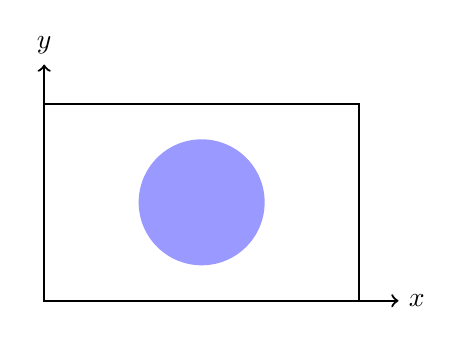
\begin{tikzpicture}
    \draw[thick] (0,0) rectangle (4,2.5);
    \fill[blue!40] (2,1.25) circle (0.8);
    \draw[->, thick] (0,0) -- (4.5,0) node[right] {$x$};
    \draw[->, thick] (0,0) -- (0,3) node[above] {$y$};
  \end{tikzpicture}
\end{frame}

\begin{frame}{The end}
  \centering
  \Large Last slide
\end{frame}

\end{document}
